\chapter{Distribuzione}
\label{chap:deploy}

Il modello di inferenza è stato rilasciato attraverso la piattaforma Microsoft Azure e anche reso fruibile per gli operatori SKF utilizzando PowerBI.
Microsoft Azure è una piattaforma Cloud che offre una suite completa di servizi e risorse per computing, storage, gestione dati, comunicazione ecc.
All'interno di questo progetto, sono stati utilizzate le seguenti risorse:
\begin{itemize}
	\item Data Factory: è uno strumento di orchestrazione per servizi di Data Integration ed esegue flussi di lavoro ETL (Extract, Transform, Load).
	\item Machine Learning: è lo strumento Azure dedicato ai servizi di Machine Learning. Mette a disposizione macchine virtuali, pipeline schedulabili, endpoint per l'inferenza, gestione dei modelli registrati ecc.
\end{itemize}

PowerBI è stato utilizzato per lo sviluppo front-end. È un software interattivo per la Data Visualization con un focus primario alla Business Intelligence. Al suo interno sono presenti numerosi connettori da cui prelevare i dati, insieme ad una serie di strumenti per aggregare, filtrare, comporre e visualizzare i dati attraverso grafici o report.

\section{Architettura}
Questa sezione è dedicata a come gli strumenti sopracitati comunicano e interagiscono tra di loro. L'architettura può essere divisa in 4 macro aree:
\begin{enumerate}
	\item \textbf{Data}: i dati sono archiviati all'interno di SQL Server e vengono aggiornati in tempo reale a seguito dell'inserimento di nuove registrazioni da parte di SKF.
	\item \textbf{Orchestrazione}: il workflow viene gestito da Data Factory il quale si occupa di richiamare l'endpoint di inferenza ad una frequenza regolare.
	\item \textbf{Training e Inferenza} sono gestiti da Azure Machine Learning. É presente una pipeline di training che consiste nel (1) processamento dati, (2) training del modello e (3) pubblicazione di esso. Il modello pubblicato genererà un endpoint di inferenza richiamabile tramite chiamate HTTP. 
	\item \textbf{Visualizzazione} dei risultati di inferenza in tempo reale attraverso PowerBI.
\end{enumerate}

\begin{figure}[t]
		
	\centering
	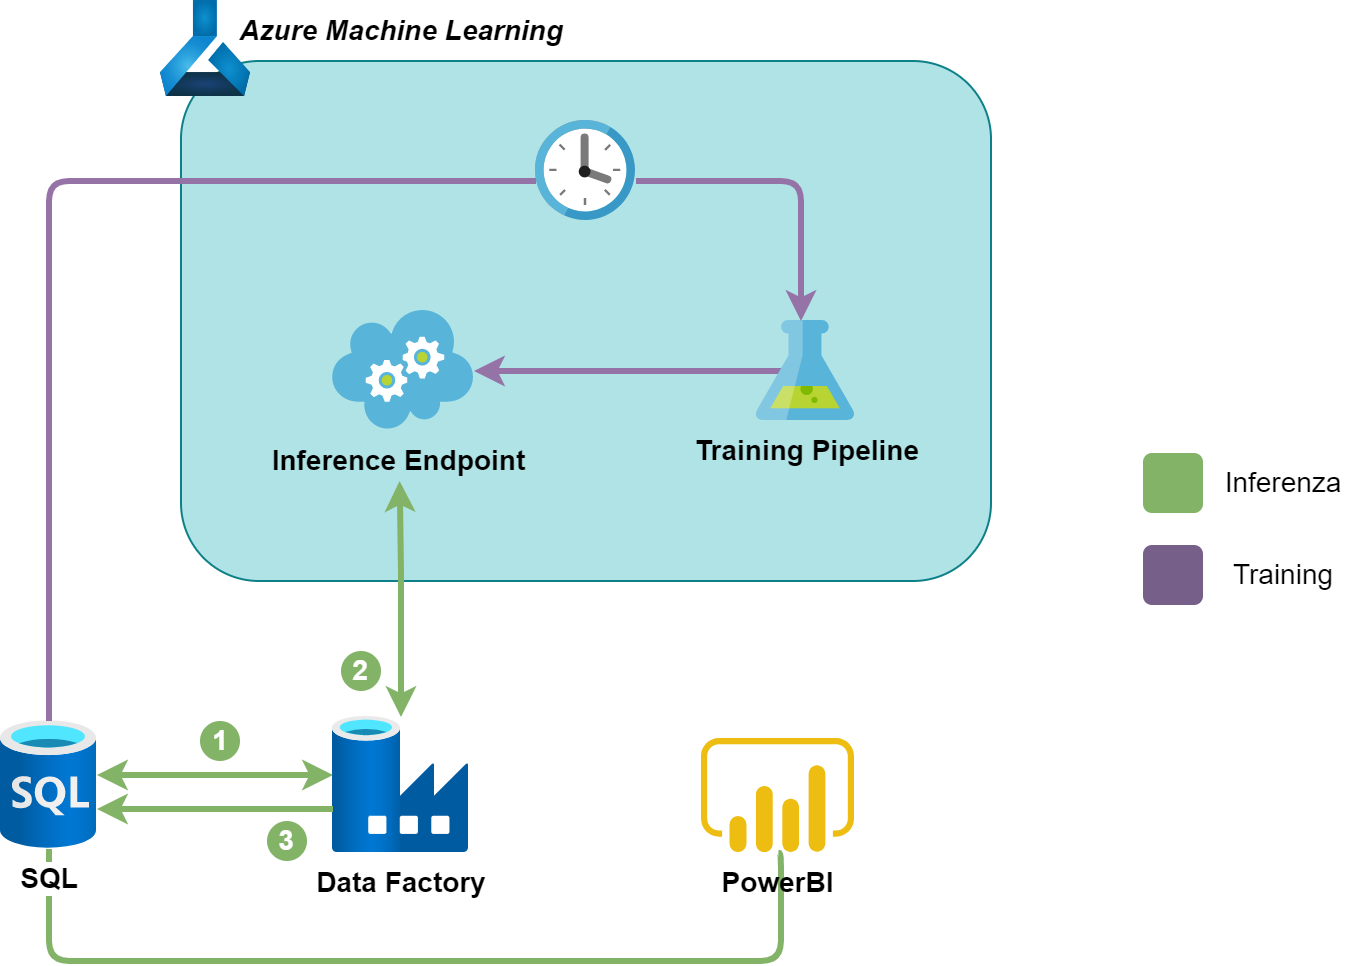
\includegraphics[width=14cm, scale=1]{images/deploy_scheme}
	\caption{Architettura Azure}
	\label{azure}
	
\end{figure}


Il flusso delle operazioni si divide invece in Training e Inferenza.

\subsubsection{Training}
Il flusso di train (in viola) è schedulato ogni mese. La pipeline di training recupera i dati da SQL server per andare a processarli e poi passarli alla funzione di allenamento del modello. L'ultimo step della pipeline riguarda la pubblicazione del modello allenato andando ad aggiornare l'endpoint di inferenza.

\subsubsection{Inferenza}
Il flusso di inferenza (in verde) è orchestrato da Data Factory il quale è stato programmato per interrogare l'archivio SQL ad una frequenza regolare. I dati vengono quindi recuperati, preparati e inclusi nella richiesta HTTP verso l'endpoint di inferenza di Azure Machine Learning. Il risultato dell'inferenza viene poi restituito a Data Factory che si occupa di salvarlo dentro il database SQL, rendendolo disponibile anche ad altri client come PowerBI. Attraverso l'utilizzo delle Direct Query, PowerBI interroga il database SQL per andare a recuperare sia i dati delle registrazioni SKF, sia il risultato di inferenza per quei dati per poi mostrarli a video.


\section{Training}
\subsection{Pipeline di Azure Machine Learning}
Il core della piattaforma Azure Machine Learning risiede nelle pipeline. Queste permettono l'esecuzione di script Python come se fossero step di esecuzione di un flusso di lavoro. Quando la pipeline viene lanciata, una richiesta di attivazione viene inoltrata al Compute Cluster associato, il quale alloca una Virtual Machine per eseguire il codice. Questo tipo di gestione On-Demand permette di utilizzare le risorse computazionali solamente quando servono, abbassando quindi i costi. Infatti, una volta terminata la pipeline, la Virtual Machine verrà deallocata dopo un periodo di inattività specificato.
La definizione della pipeline viene effettuata utilizzando l'SDK di AzureML. 
I parametri richiesti sono (1) il nome del Compute Cluster su cui eseguire il flusso di lavoro e (2) il nome dell'environment. L'environment è un ambiente di lavoro che contiene informazioni sulle dipendenze e sulle versioni dei pacchetti, librerie o dell'interprete Python necessari alla corretta esecuzione del codice. Gli environment sono definiti utilizzando un Dockerfile e registrati su Azure Machine Learning.
Gli step della pipeline sono invece definiti dal percorso allo script del file Python locale, i parametri di input e i parametri di output. Condividono lo stesso spazio di archiviazione, di conseguenza per passare dati tra gli step è necessario andare a salvare su file questi dati e valorizzare i vari input e output con i percorsi a questi.
A questo punto la pipeline è completa e può essere pubblicata su Azure Machine Learning per essere poi schedulata ad una cadenza regolare.

\subsection{Pipeline di training SKF}
In questa sezione vengono descritti i flussi di lavoro della pipeline per il training di SKF.
\begin{enumerate}
	\item La tabella \textit{Dataset} contiene al suo interno le registrazioni dei sensori del macchinario M1 di SKF. La struttura dati, a questo punto del flusso di lavoro, è ancora grezza: ogni riga della tabella corrisponde ad un'unica osservazione per uno specifico sensore. Attraverso l'uso di un connettore, questi dati vengono prelevati dalla tabella SQL e trasformati in un Pandas Data Frame.
	\item Il secondo step della pipeline, chiamato \textit{Prepare Data}, si occupa di processare i dati come mostrato nel capitolo \ref{chap:skf}. Il nuovo Data Frame viene salvato su file per essere letto dal prossimo passaggio.
	\item Il terzo step, \textit{Train Model}, si occupa del training del modello. Il modello viene recuperato dall'archivio di Azure Machine Learning il quale contiene una lista di tutti i modelli registrati. In questo caso il modello registrato corrisponde al miglior modello ottenuto dal Model Selection non supervisionato che viene eseguito in locale. La scelta di non automatizzare anche il Model Selection risiede nel fatto che quest'algoritmo deve essere eseguito solamente una volta in quanto i dati di uno specifico macchinario non cambiano particolarmente tanto nel tempo, salvo grossi interventi di manutenzione che implicano la sostituzione di tutti i sensori. Recuperato il modello dall'archivio e letto il dataset processato, si può eseguire il training. A fine di questo passaggio, il modello trainato viene salvato su file per renderlo disponibile all'ultimo step.
	\item Il quarto step, \textit{Publish Model as Endpoint}, si occupa di andare a registrare il modello trainato nell'archivio di Azure Machine Learning, consentendo quindi di aggiornare la versione del modello corrente con una nuova. Infine viene anche pubblicato, oppure aggiornato, l'endpoint di inferenza con il nuovo modello.
\end{enumerate}


\begin{figure}[t]
	\centering
	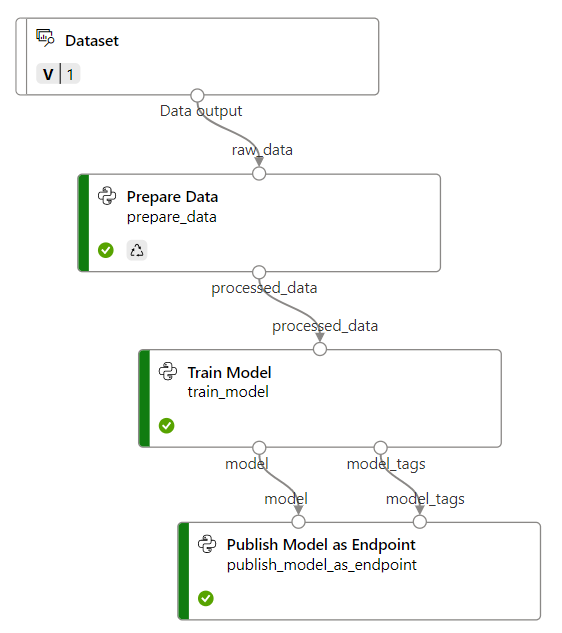
\includegraphics[width=10cm, scale=1]{images/pipeline}
	\caption{Pipeline di Training}
	\label{pipeline-training}
\end{figure}

\section{Inferenza}
\subsection{Pipeline di Azure Data Factory}
Come per la piattaforma Machine Learning, Azure Data Factory si basa sulle pipeline, ma che a differenza del primo non sono definite tramite l'SDK e non eseguono script Python, ma si utilizza il pannello di controllo Data Factory Studio per impostare i passaggi e le operazioni da eseguire andando a comporre il flusso di lavoro con un approccio drag-and-drop.
La piattaforma mette a disposizioni numerose operazioni come step della pipeline: recuperò dati; copia dati; esecuzione di script, stored procedure; chiamate http, azure functions e molto altro. 
Gli step sono collegati tramite flussi condizionali sulla base se concludono correttamente o meno ed è possibile passare dati tra i vari step.
Un'altra differenza con le pipeline di Azure Machine Learning è che non bisogna definire l'environment o il Compute Cluster ma è tutto eseguito sulle risorse computazionali di Azure On-Demand.
Infine, la pipeline può essere pubblicata e schedulata a cadenza regolare per automatizzarne l'esecuzione.
\subsection{Pipeline di inferenza SKF}
In questa sezione sono definiti gli step della pipeline di inferenza.
\begin{enumerate}
	\item Il primo step si occupa di prelevare dal database SQL i dati appena inseriti da SKF che contengono le ultime registrazione dei sensori di un macchinario. 
	\item Il secondo step richiama l'endpoint di inferenza pubblicato dalla pipeline di training. È una chiamata POST nella quale al suo interno vengono inclusi i dati dello step 1.
	\item Infine il terzo step si occupa si salvare su database SQL, attraverso il richiamo di una Stored Procedure, il risultato dell'inferenza. Rendendolo così disponibile a tutti quei client che ne necessitano l'utilizzo, come PowerBI
\end{enumerate}

\begin{figure}[t]
	\centering
	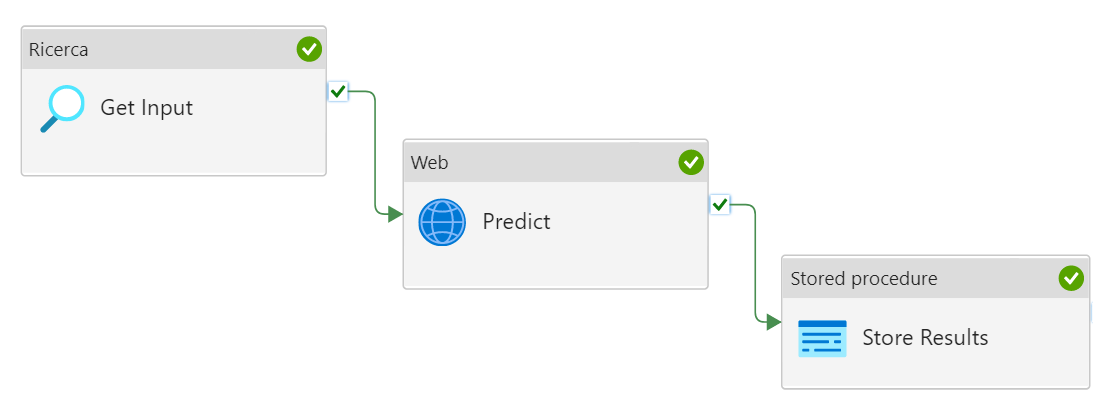
\includegraphics[width=10cm, scale=1]{images/pipeline-inference}
	\caption{Pipeline di Inferenza}
	\label{pipeline-inferenza}
\end{figure}

\section{Dashboard}
L'ultimo elemento dell'architettura è PowerBI. Come introdotto a inizio capitolo, è un software interattivo per la Data Visualization che offre diversi connettori da cui prelevare i dati. Uno di questi è il Direct Query: questo strumento permette di collegarsi direttamente all'origine dei dati ed interrogarla On-Demand. È un modo particolarmente efficace di recuperare i dati quando si ha a disposizione un archivio molto grande e non si vuole scaricarli tutti in locale; questo metodo consente infatti di ottenere i dati già trasformati e raggruppati, pronti per essere mostrati, riducendo cosi il carico di lavoro e la quantità di dati trasferiti. È però necessario andare a schedulare un refresh dei dati in modo da mostrare report sempre aggiornati. 
Attraverso questo metodo si ha quindi un collegamento diretto al database SQL utilizzato per andare a prelevare i dati salvati dalla pipeline di inferenza.
L'interfaccia pensata per gli operatori di SKF risiede in un semplice grafico a linee con delle barre verticali rosse per indicare l'anomalia in uno specifico timestamp. Per questo tipo di report, Direct Query è indubbiamente la scelta migliore di recuperare i dati.  


\begin{figure}[t]
	\centering
	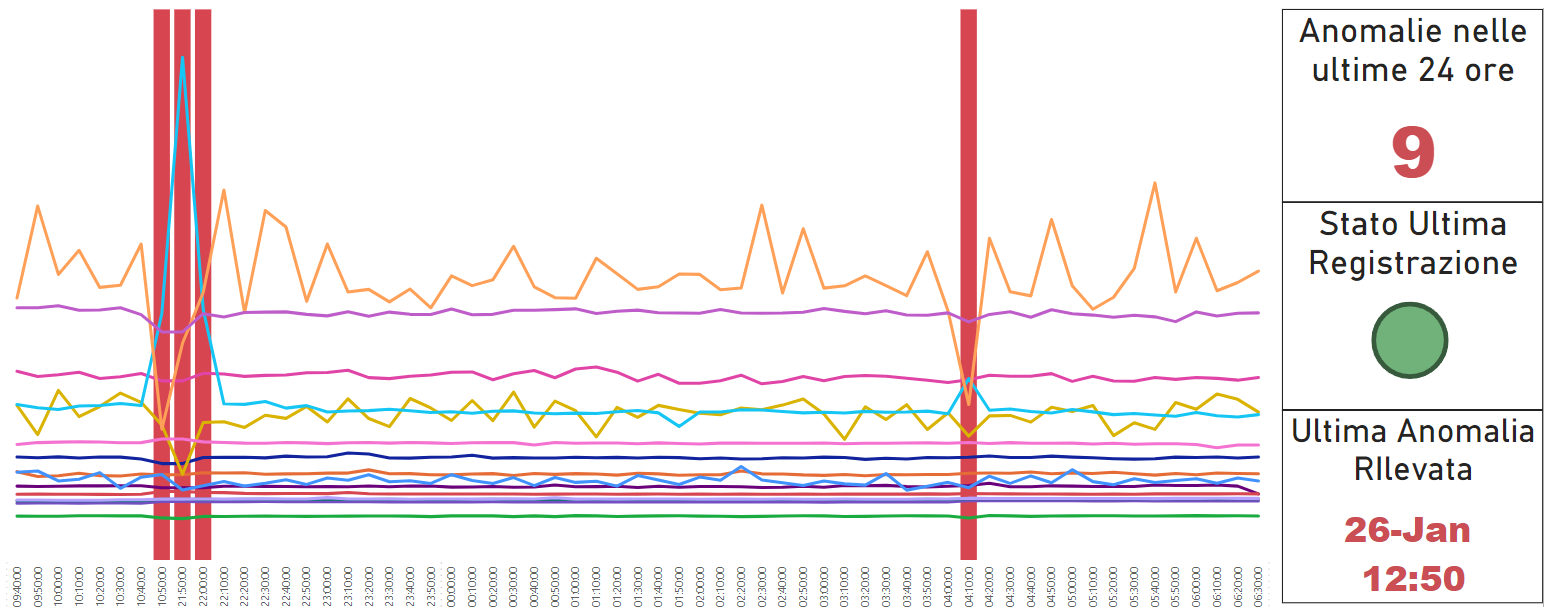
\includegraphics[width=14cm, scale=1]{images/powerbi}
	\caption{Dashboard PowerBI}
	\label{powerbi}
\end{figure}

In figura \ref{powerbi} è presente il grafico appena descritto. È possibile notare, all'interno delle barre verticali rosse, come ci siano dei picchi o valori anomali per alcune delle linee orizzontali, ovvero i sensori del macchinario. Sulla destra, invece, alcune informazioni circa l'andamento del sistema. 